%% =============================================================================
%%  ECON 580 Senior Thesis — Status Update Presentation
%%  Author:  Alejandro De La Torre
%%  Date:    March 26, 2026
%% =============================================================================

\documentclass[10pt]{beamer}

%% ---- Theme (minimal; no external package required) -------------------------
\usetheme{default}
\usecolortheme{dove}          % gray-scale, clean
\setbeamertemplate{navigation symbols}{}  % remove nav icons
\setbeamertemplate{footline}[frame number]
\setbeamertemplate{itemize items}[circle]
\setbeamertemplate{enumerate items}[default]
\setbeamercolor{frametitle}{fg=black}
\setbeamercolor{title}{fg=black}
\setbeamercolor{structure}{fg=black}
\setbeamerfont{frametitle}{series=\bfseries}

%% ---- Packages --------------------------------------------------------------
\usepackage{graphicx}
\usepackage{booktabs}
\usepackage{amsmath}
\usepackage{xcolor}
\usepackage{hyperref}
\usepackage{array}
\usepackage{microtype}

%% ---- Figure path -----------------------------------------------------------
\graphicspath{{images/}}

%% ---- Custom colors ---------------------------------------------------------
\definecolor{fdablue}{RGB}{0, 60, 120}
\definecolor{alertred}{RGB}{180, 30, 30}

%% ---- Helpers ---------------------------------------------------------------
\newcommand{\src}[1]{{\tiny\textcolor{gray}{#1}}}

%% ---- Title metadata --------------------------------------------------------
\title[PDUFA \& CS Approvals]%
      {PDUFA and Controlled Substance Approvals\\[0.3em]
       \large Progress Report}
\subtitle{ECON 580 Senior Thesis --- 3rd Status Update}
\author{Alejandro De La Torre}
\date{March 26, 2026}
\institute{Department of Economics\\University of Wisconsin--Madison}

%% =============================================================================
\begin{document}
%% =============================================================================

%% ---- Title slide -----------------------------------------------------------
\begin{frame}
  \titlepage
\end{frame}

%% =============================================================================
\section{Research Question and Overview}
%% =============================================================================

\begin{frame}[t]{Research Question}
  \textbf{Core question:}
  \begin{quote}
    Did the Prescription Drug User Fee Act (PDUFA, 1992) increase the share of
    FDA-approved drugs that are DEA-scheduled controlled substances?
  \end{quote}

  \medskip
  \textbf{Motivation:}
  \begin{itemize}
    \item PDUFA introduced industry-funded user fees that expanded FDA review
          capacity and increased approval throughput
    \item Faster reviews $\Rightarrow$ more drugs approved sooner --- but did
          this disproportionately benefit drugs with \textbf{abuse potential}?
    \item Conceptual channel: regulatory acceleration $\to$ greater CS supply
          $\to$ downstream diversion and misuse risk
  \end{itemize}

  \medskip
  \textbf{This presentation:} descriptive findings, first-pass event study
  results, honest accounting of problems, and paths forward.
\end{frame}

\begin{frame}[t]{Roadmap}
  \begin{enumerate}
    \item What PDUFA is --- and what it is not
    \item Data construction and sample
    \item Descriptive results (8 figures)
    \item Event study results (5 figures)
    \item Problems and limitations (6 issues)
    \item Where the thesis stands
    \item Paths forward and discussion
  \end{enumerate}
\end{frame}

%% =============================================================================
\section{What Are User Fees?}
%% =============================================================================

\begin{frame}[t]{What PDUFA Does}
  \begin{itemize}
    \item Enacted October 1992; reauthorized every 5 years (now PDUFA VII,
          through 2027)
    \item Authorizes FDA to collect fees from firms submitting drug applications
    \item Fees fund \textbf{FDA staffing} to review applications faster ---
          not specific approval decisions
    \item \textbf{Three fee types:}
          \begin{itemize}
            \item Application fee ($\approx$\$4M for a full NDA with clinical
                  data)
            \item Annual establishment fee
            \item Annual product fee
          \end{itemize}
    \item Fees are \textbf{uniform} --- same rate regardless of drug type,
          therapeutic area, or schedule status
    \item \alert{Key point:} fees are not scaled to profitability, revenue
          potential, or abuse/diversion risk
  \end{itemize}
\end{frame}

\begin{frame}[t]{What User Fees Are NOT (1/2)}
  \begin{center}
    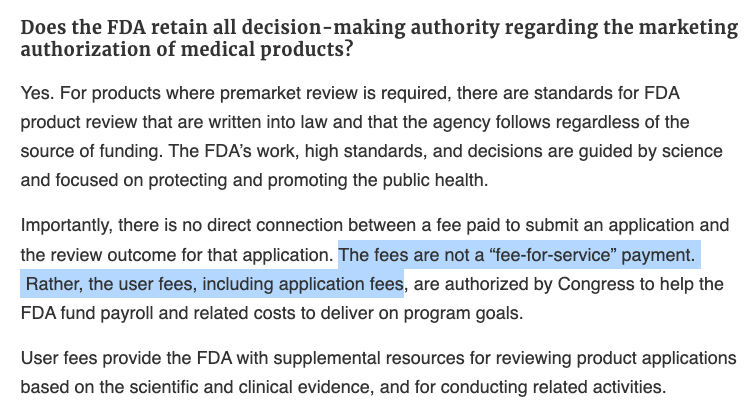
\includegraphics[width=0.88\textwidth]{user-fees_goal.png}
  \end{center}
  \medskip
  \src{Source: FDA PDUFA program documentation}\\[0.5em]
  The FDA is explicit: user fees are \textbf{not ``fee-for-service''} payments.
  They fund payroll and review capacity, not specific approval decisions.
\end{frame}

\begin{frame}[t]{What User Fees Are NOT (2/2)}
  \begin{center}
    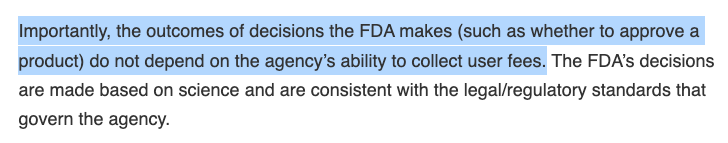
\includegraphics[width=0.88\textwidth]{user-fees_outcome.png}
  \end{center}
  \medskip
  \src{Source: FDA PDUFA program documentation}\\[0.5em]
  \textit{``The outcomes of decisions the FDA makes (such as whether to approve
  a product) do not depend on the agency's ability to collect user fees.''}
\end{frame}

\begin{frame}[t]{Critical Institutional Detail: ANDAs Not Covered Until 2012}
  \begin{itemize}
    \item PDUFA (1992) applied to \textbf{NDAs and BLAs only} --- new drugs
          and biologics
    \item Generic drug applications (ANDAs) got their own user fee program,
          \textbf{GDUFA}, only in \alert{2012}
    \item \textbf{This matters enormously because:}
          \begin{itemize}
            \item 86.6\% of controlled substance approvals in our sample are
                  \textbf{ANDAs}
            \item These were not subject to PDUFA user fees for the first 20
                  years
            \item Top CS sponsors are all generic manufacturers
          \end{itemize}
    \item \alert{Implication:} the ``user fees create incentives'' channel does
          \textbf{not} operate through the pathway where most CS action occurs
    \item If anything, GDUFA (2012) is the more relevant policy shock for the
          generics-as-CS story
  \end{itemize}
\end{frame}

%% =============================================================================
\section{Data and Sample}
%% =============================================================================

\begin{frame}[t]{Data Sources}
  \begin{itemize}
    \item \textbf{FDA: Drugs@FDA} --- all approved drug applications (NDA,
          ANDA, BLA), downloaded March 2026
          \begin{itemize}
            \item 12 relational tables; submission events keyed by
                  \texttt{ApplNo + SubmissionType + SubmissionNo}
            \item Covers approved applications only (failed/withdrawn not
                  observed)
          \end{itemize}
    \item \textbf{DEA: Controlled Substance Schedules} --- official scheduling
          classifications (Schedules I--V), March 2026
          \begin{itemize}
            \item Linked at the \textbf{active ingredient} level
            \item If any ingredient matches a DEA-scheduled substance, the drug
                  is flagged
            \item \alert{Current schedules, not historical} --- a limitation
                  we will return to
          \end{itemize}
    \item \textbf{Conservative definition:} only confident, exact DEA schedule
          matches count as controlled substances
  \end{itemize}
\end{frame}

\begin{frame}[t]{Sample Construction}
  \begin{center}
  \begin{tabular}{lrr}
    \toprule
    Step & Observations & Dropped \\
    \midrule
    Full FDA backbone (all submission events) & 191,266 & --- \\
    Keep original approved (ORIG + AP) & 26,268 & 164,998 \\
    Deduplicate by application (earliest date) & 26,076 & 192 \\
    Drop 2026 partial year + null dates & 25,908 & 168 \\
    \midrule
    \textbf{Final sample} & \textbf{25,908} & --- \\
    \bottomrule
  \end{tabular}
  \end{center}
  \medskip
  \begin{itemize}
    \item One row per unique approved drug application (\texttt{ApplNo})
    \item Year range: 1939--2025
    \item Unit: the \textbf{first original approval} for each application
  \end{itemize}
\end{frame}

\begin{frame}[t]{Sample Overview}
  \begin{columns}[t]
    \column{0.5\textwidth}
    \textbf{By application type:}
    \medskip
    \begin{tabular}{lr}
      \toprule
      Type & N \\
      \midrule
      ANDA (generic)   & 19,022 (73.4\%) \\
      NDA (new drug)   & 5,277  (20.4\%) \\
      BLA (biologic)   & 460    (1.8\%)  \\
      Other/unknown    & 1,149  (4.4\%)  \\
      \bottomrule
    \end{tabular}
    \column{0.5\textwidth}
    \textbf{Controlled substances (CS = 2,067, 8.0\%):}
    \medskip
    \begin{tabular}{lr}
      \toprule
      Schedule & N \\
      \midrule
      II   & 994 (48.1\%) \\
      IV   & 769 (37.2\%) \\
      III  & 189 (9.1\%)  \\
      V    & 108 (5.2\%)  \\
      I    &  7  (0.3\%)  \\
      \bottomrule
    \end{tabular}
  \end{columns}
\end{frame}

\begin{frame}[t]{Key Fact: Controlled Substances Are Overwhelmingly Generics}
  \begin{itemize}
    \item Among 2,067 CS approvals:
          \begin{itemize}
            \item \textbf{1,790 are ANDAs (86.6\%)}
            \item Only \textbf{276 are NDAs (13.4\%)}
          \end{itemize}
    \item CS share \textit{within} type:
          \begin{itemize}
            \item Among ANDAs: 9.4\% are CS
            \item Among NDAs: 5.2\% are CS
          \end{itemize}
    \item Top 20 sponsors of CS approvals are \textbf{all generic manufacturers}
          (Watson, Hikma, Sandoz, Barr, Qualitest, Mallinckrodt, \ldots)
    \item No major innovator pharmaceutical companies appear in the top 20
    \item \alert{What this tells us:} the CS approval story is a
          \textbf{generic drug entry story}, not a novel-drug-development story
    \item That is a \textbf{Hatch-Waxman (1984) story}, not a PDUFA story
  \end{itemize}
\end{frame}

%% =============================================================================
\section{Descriptive Results}
%% =============================================================================

\begin{frame}[t]{Total Drug Approvals Over Time}
  \begin{center}
    
\includegraphics[width=\textwidth]{fig_annual_approvals.png}
  \end{center}
  \vfill
  \src{Massive growth in total approvals, especially after Hatch-Waxman (1984) ---
  the generic-drug entry mechanism. This is the denominator explosion.}
\end{frame}

\begin{frame}[t]{Approvals by Application Type}
  \begin{center}
    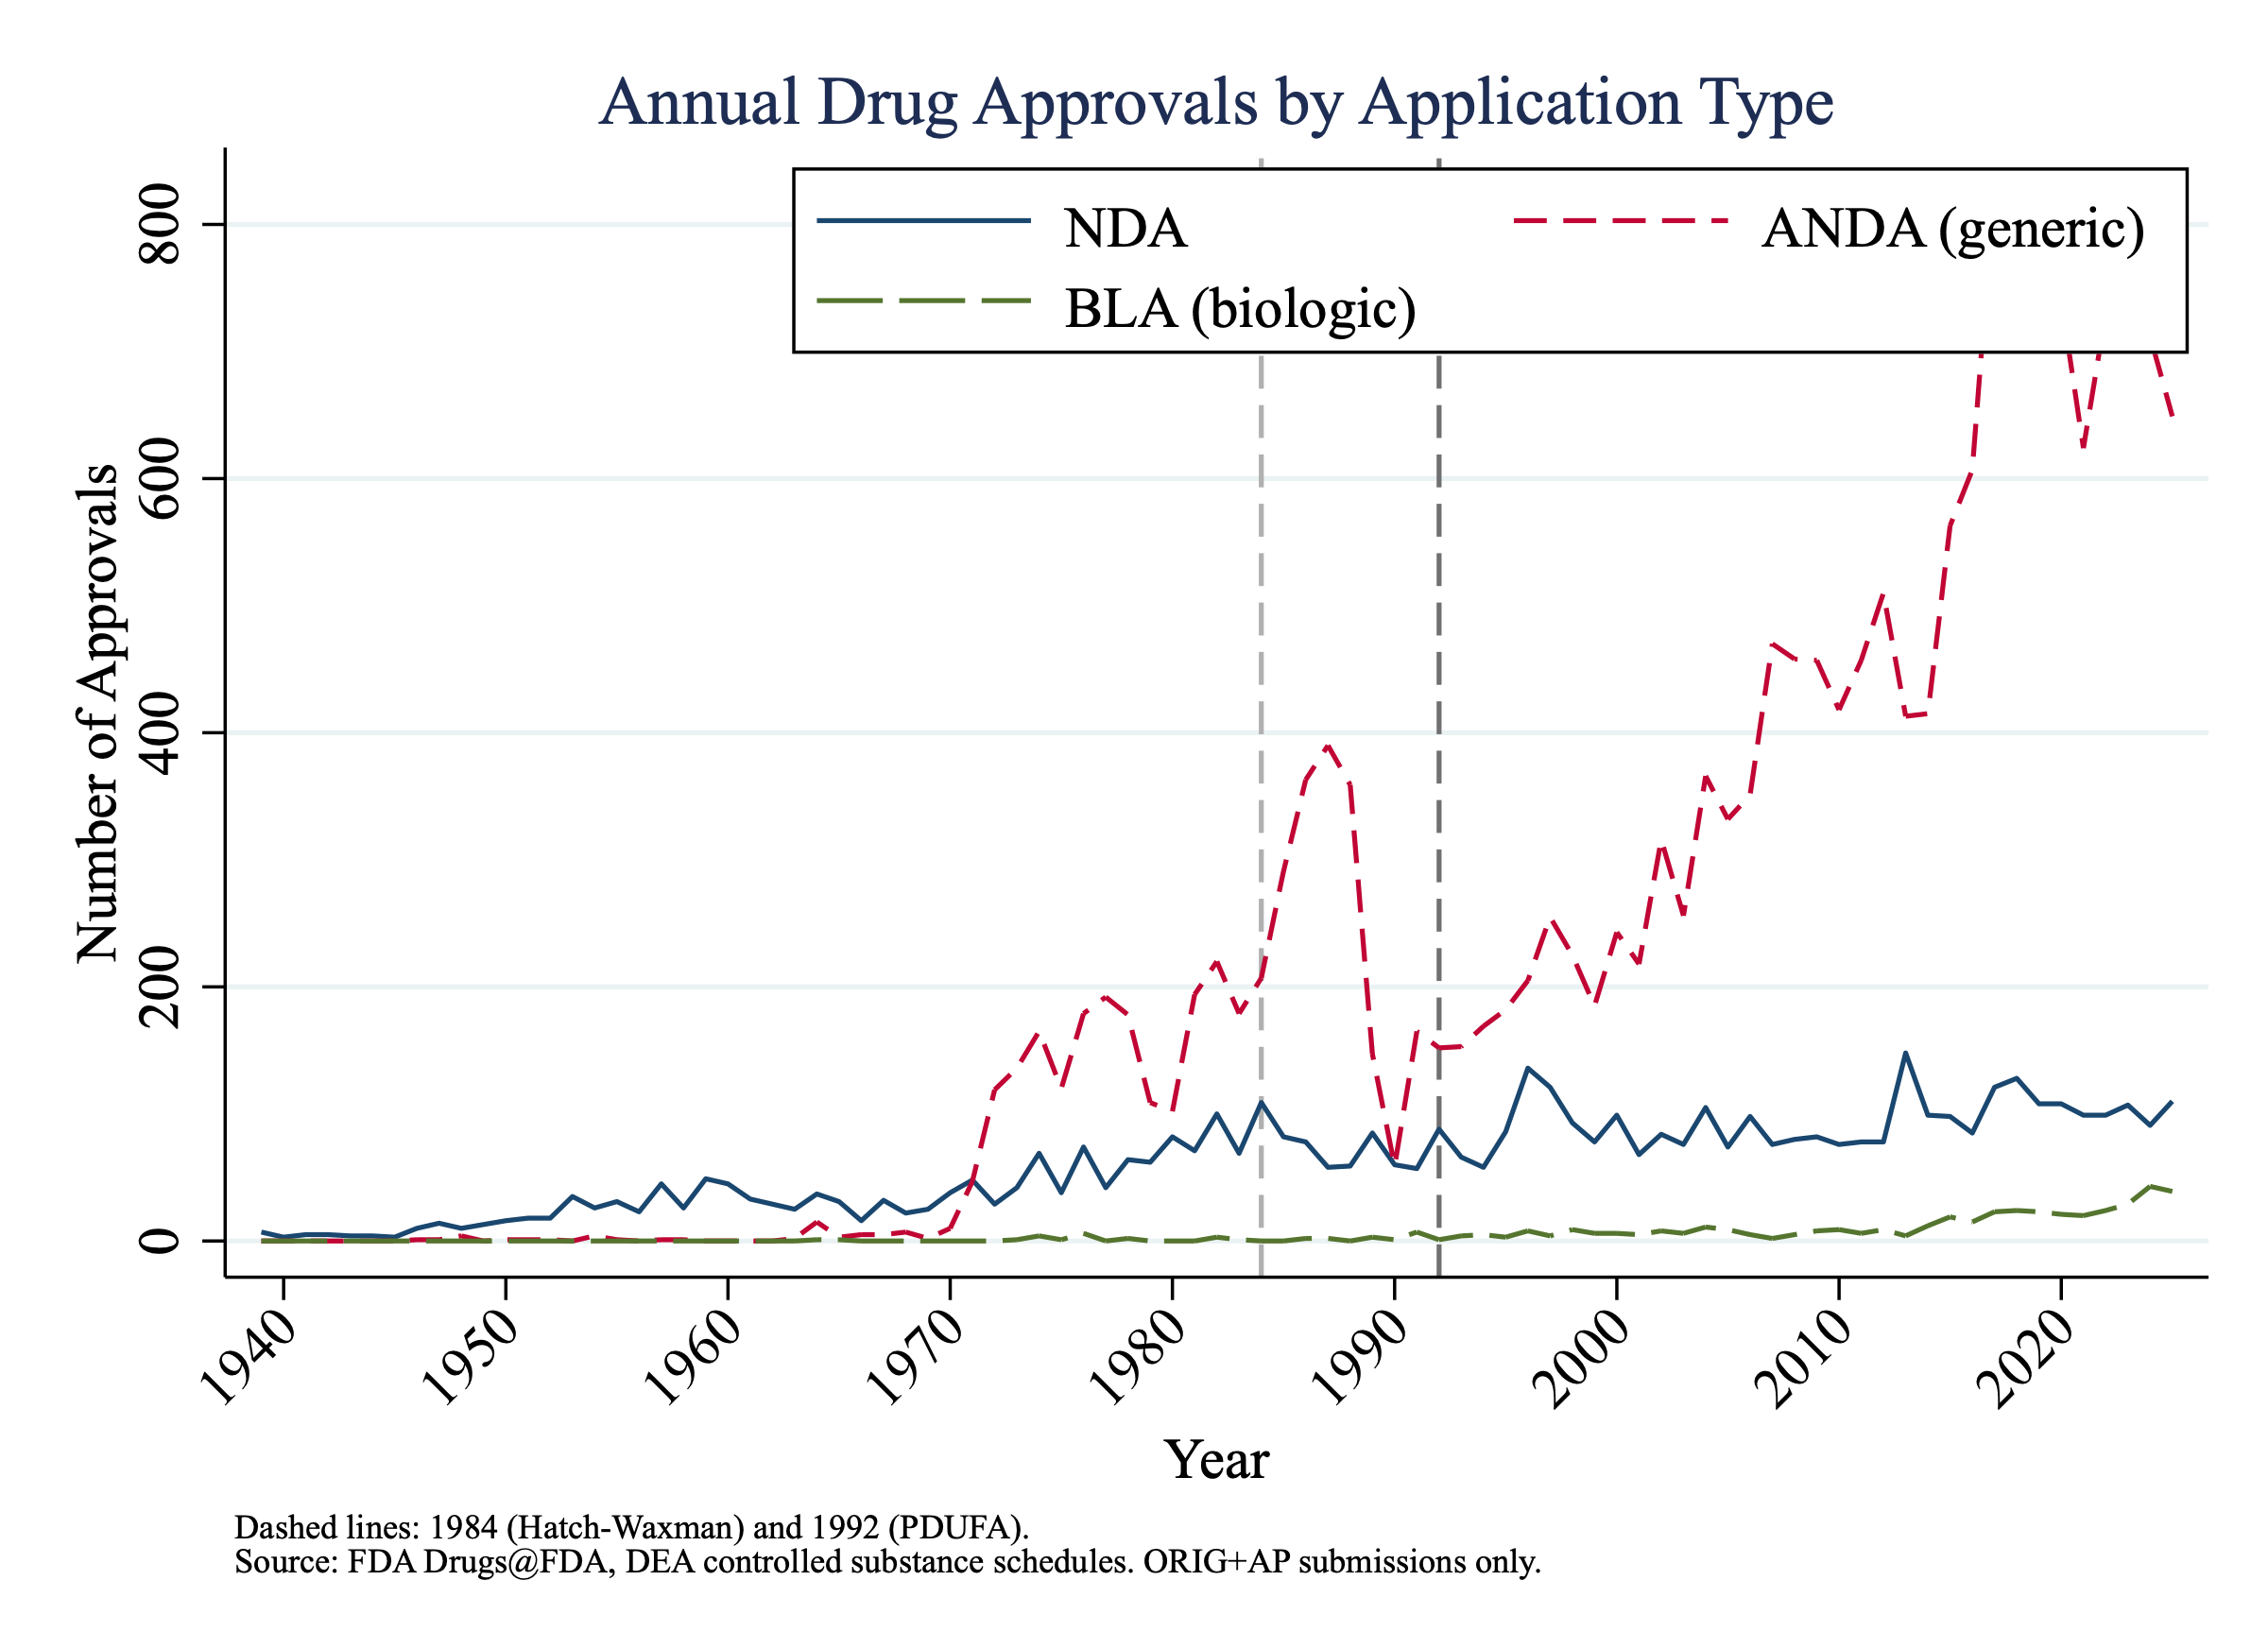
\includegraphics[width=\textwidth]{fig_annual_approvals_by_appltype.png}
  \end{center}
  \vfill
  \src{Growth is almost entirely ANDA-driven. NDA approvals are relatively flat.
  BLAs appear only after 1982. The composition of the approval pool changed
  fundamentally after Hatch-Waxman.}
\end{frame}

\begin{frame}[t]{Annual Controlled Substance Approvals (Count)}
  \begin{center}
    
\includegraphics[width=\textwidth]{fig_annual_cs_approvals.png}
  \end{center}
  \vfill
  \src{CS approvals grew in absolute terms --- from low single digits pre-1970
  to 40--70/year recently. But total approvals grew even faster.}
\end{frame}

\begin{frame}[t]{Share of Approvals That Are Controlled Substances}
  \begin{center}
    
\includegraphics[width=\textwidth]{fig_cs_share.png}
  \end{center}
  \vfill
  \src{\textbf{Main descriptive figure.} CS share was highest in the 1940s--1970s.
  It has been on a general decline since the early 1980s.
  No visible upward break at 1992 (PDUFA).}
\end{frame}

\begin{frame}[t]{CS Share by Application Type (NDA vs.\ ANDA)}
  \begin{center}
    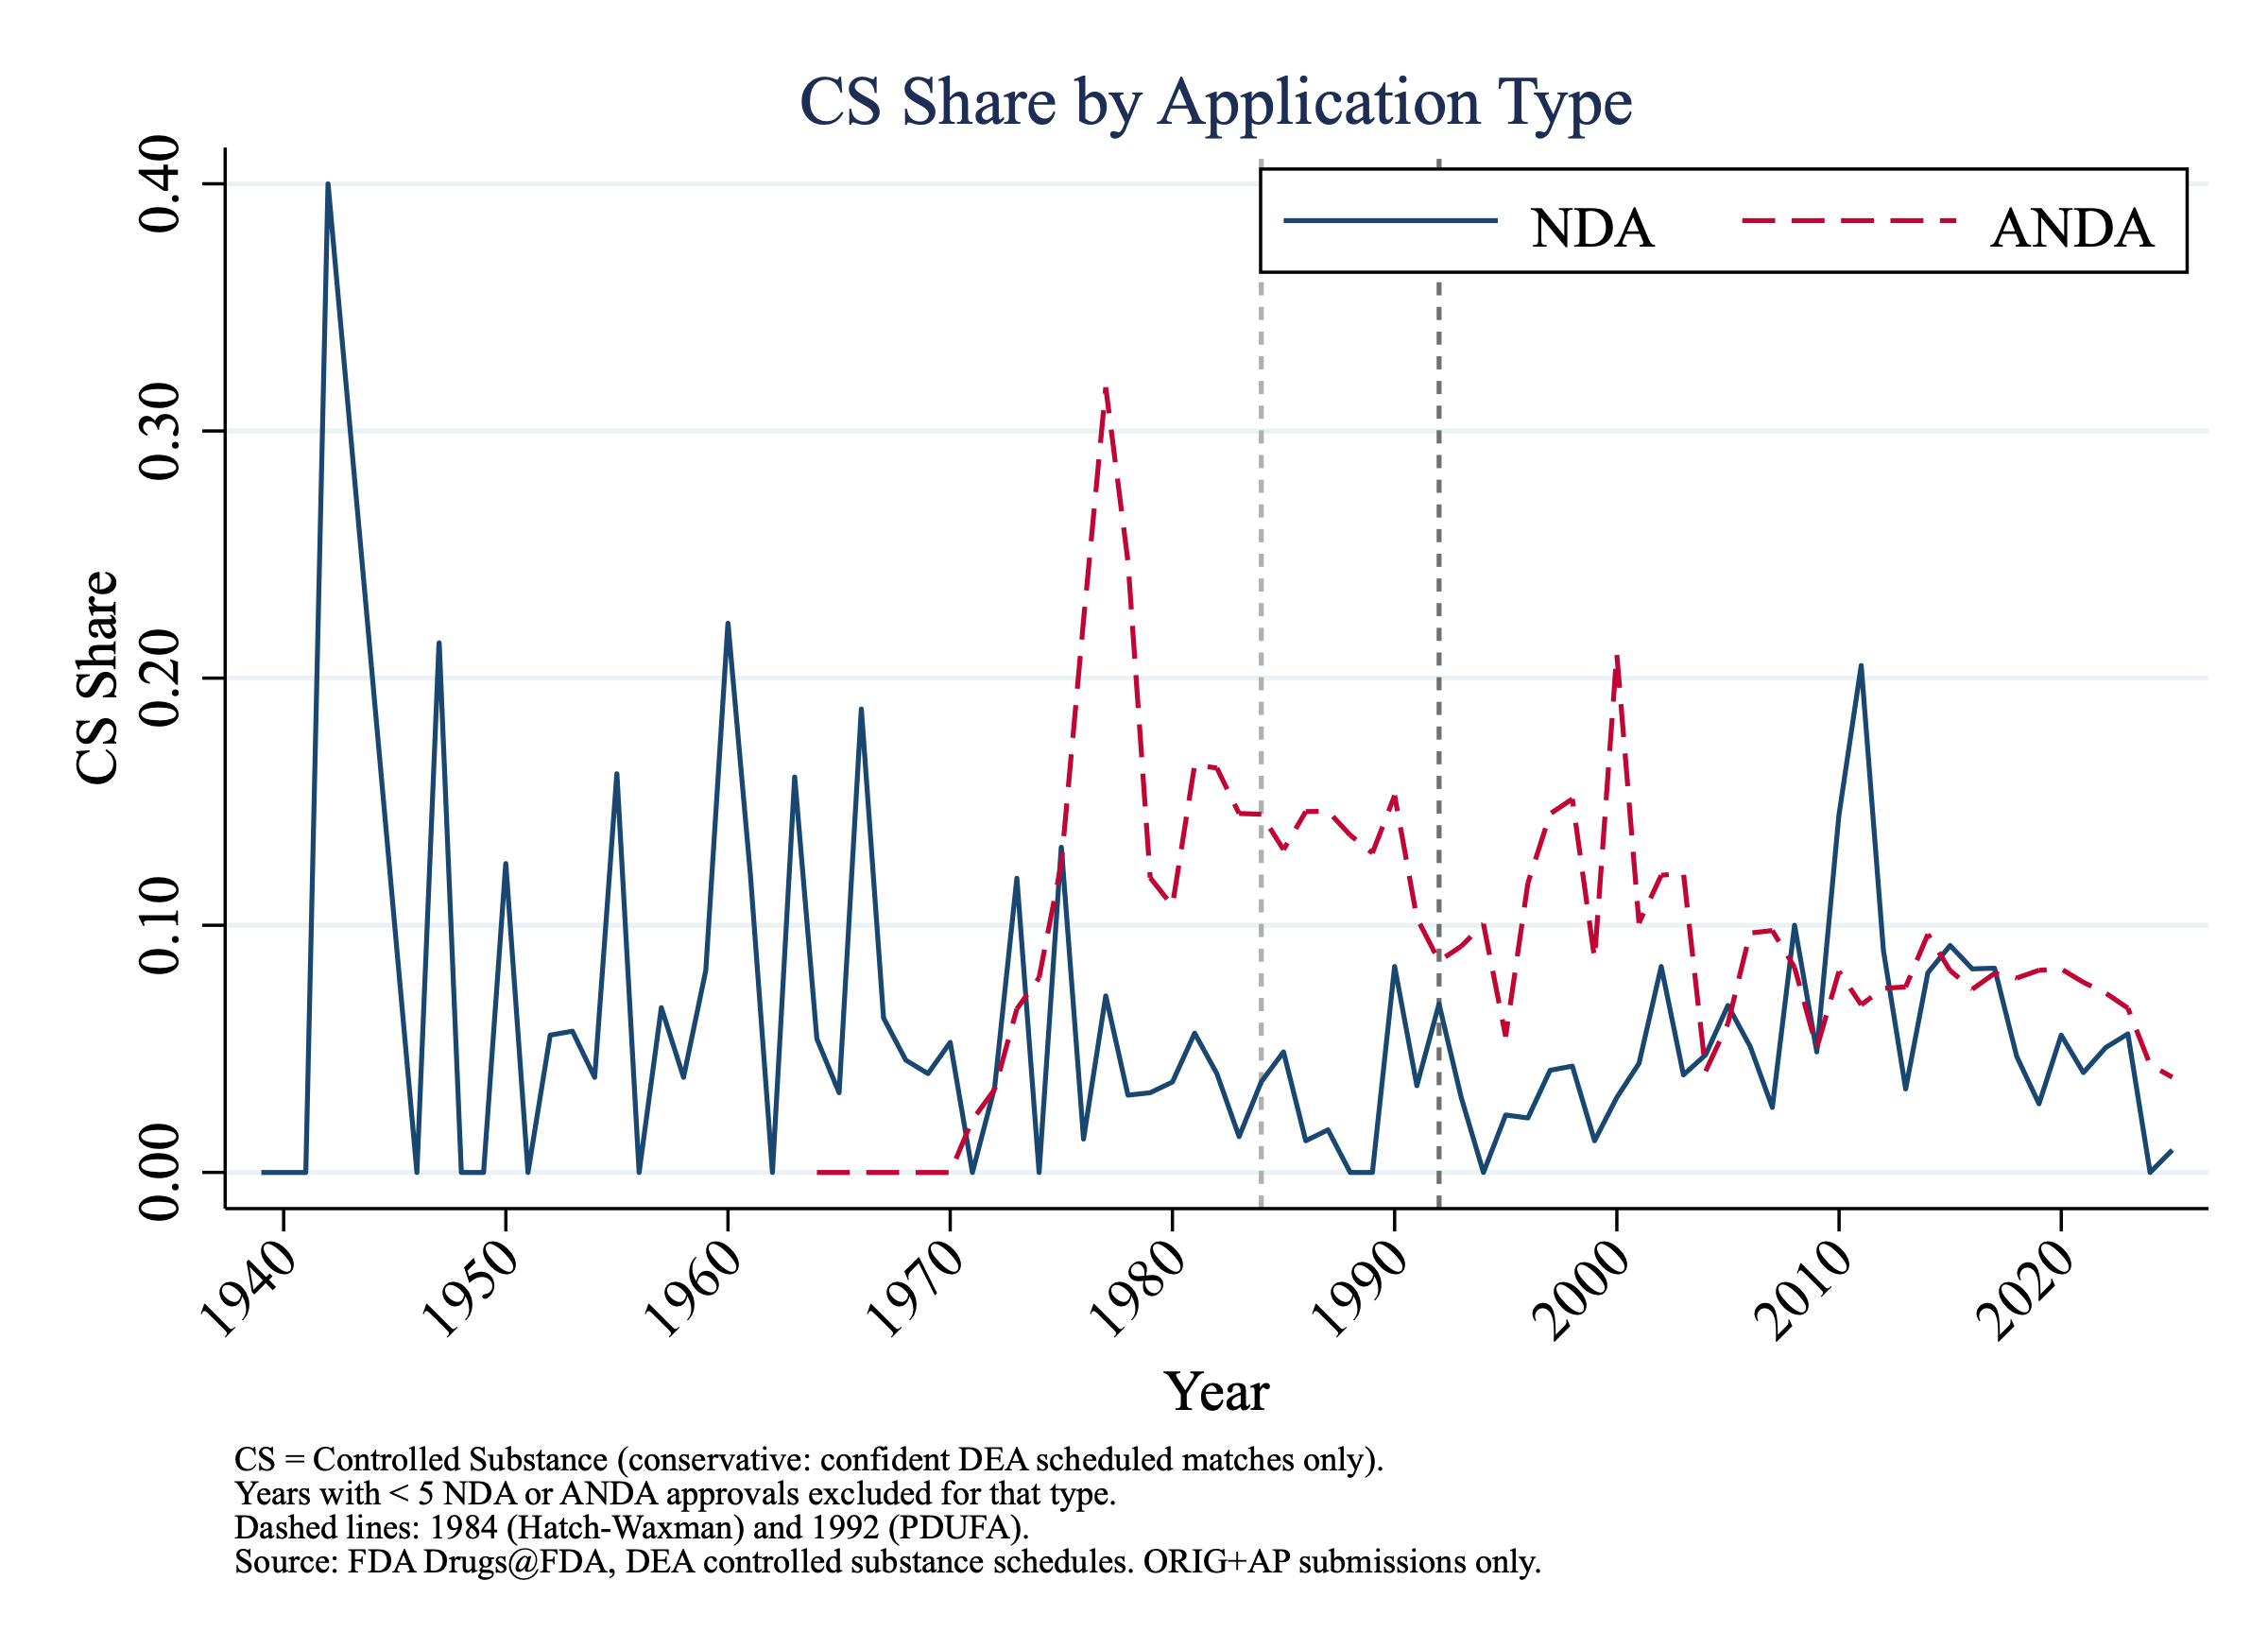
\includegraphics[width=\textwidth]{fig_cs_share_by_appltype.png}
  \end{center}
  \vfill
  \src{NDA CS share is volatile but generally higher than ANDA CS share.
  ANDA CS share spikes in early 1980s (Hatch-Waxman era) then settles
  around 5--10\%. Years with fewer than 5 approvals of a given type excluded.}
\end{frame}

\begin{frame}[t]{Controlled Substance Approvals by DEA Schedule}
  \begin{center}
    
\includegraphics[width=\textwidth]{fig_cs_by_schedule.png}
  \end{center}
  \vfill
  \src{Schedule II and IV dominate. Schedule II (opioids, stimulants) has grown
  notably since $\approx$2005. The growth in Schedule II generics drives most
  of the absolute CS approval increase.}
\end{frame}

\begin{frame}[t]{Mean CS Share by PDUFA Era}
  \begin{center}
    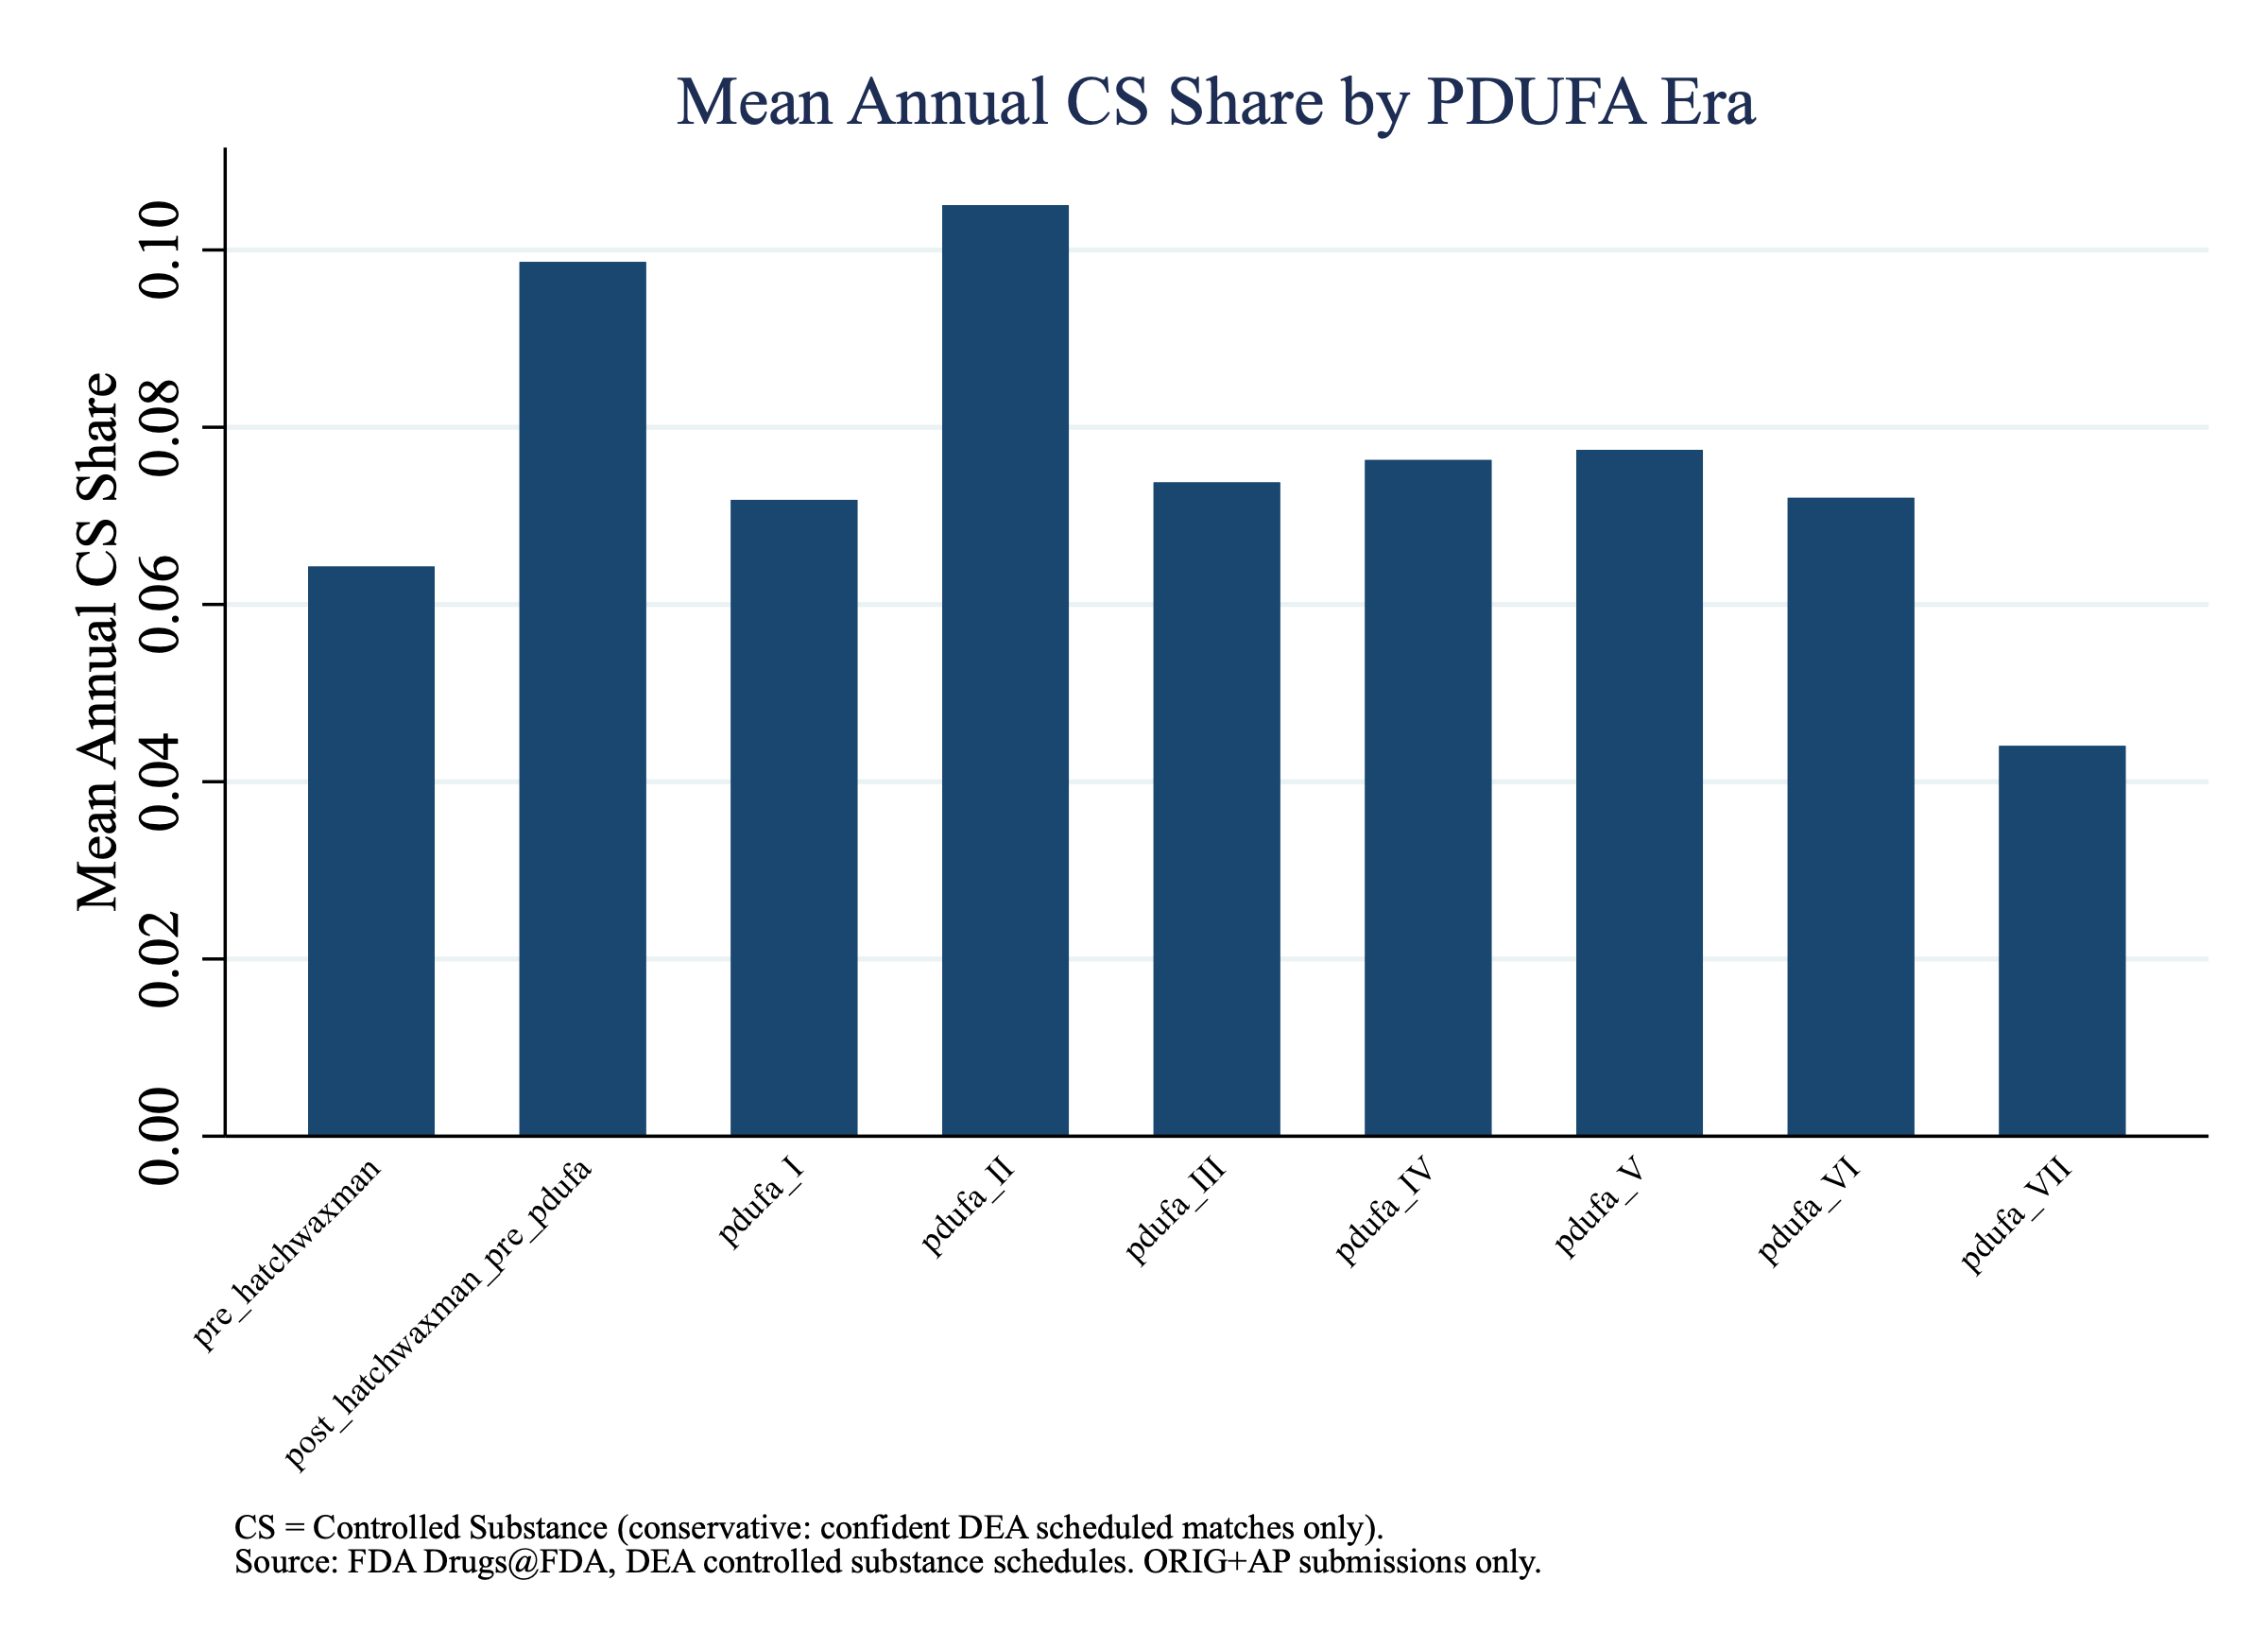
\includegraphics[width=\textwidth]{fig_cs_share_pdufa_eras.png}
  \end{center}
  \vfill
  \src{CS = Controlled Substance. No monotonic increase across PDUFA eras.
  PDUFA VII (2023+) has the lowest mean CS share. PDUFA II had the highest
  among PDUFA periods --- likely driven by the early generic opioid wave.}
\end{frame}

\begin{frame}[t]{Conservative vs.\ Broad CS Definition}
  \begin{center}
    
\includegraphics[width=\textwidth]{fig_cs_share_broad_vs_conservative.png}
  \end{center}
  \vfill
  \src{The two definitions track closely. The conservative measure
  (confident DEA matches only) is not systematically missing a large
  set of borderline cases. Definition choice does not drive the trend.}
\end{frame}

\begin{frame}[t]{Pre-PDUFA vs.\ Post-PDUFA Summary}
  \begin{columns}[t]
    \column{0.5\textwidth}
    \textbf{Pre-PDUFA (1939--1992):}
    \begin{itemize}
      \item Avg.\ 135 approvals/year
      \item Avg.\ $\approx$13 CS approvals/year
      \item CS share: $\approx$9.6\%
    \end{itemize}
    \bigskip
    \column{0.5\textwidth}
    \textbf{Post-PDUFA (1993--2025):}
    \begin{itemize}
      \item Avg.\ 564 approvals/year
      \item Avg.\ $\approx$41 CS approvals/year
      \item CS share: $\approx$7.3\%
    \end{itemize}
  \end{columns}
  \bigskip
  \begin{block}{Bottom line}
    CS approvals tripled in raw count. CS \textit{share} fell.
    Total approvals quadrupled. The ANDA explosion inflated the denominator
    faster than the numerator.
  \end{block}
\end{frame}

%% =============================================================================
\section{Event Study Results}
%% =============================================================================

\begin{frame}[t]{Event Study Design}
  \begin{itemize}
    \item \textbf{Design:} interrupted time series (ITS) centered on
          PDUFA enactment (1992)
    \item Annual data, \textbf{1970--2025} (pre-1970 dropped: tiny
          denominators, very volatile)
    \item \textbf{Reference year:} 1991 (event time = $-1$)
    \item \textbf{End-caps:} event time $\le -20$ and $\ge +30$ binned
    \item \alert{No cross-sectional variation} --- single national time series
    \item \textbf{Cannot} identify a causal treatment effect; no untreated units
    \item Results are descriptive policy diagnostics, not causal estimates
  \end{itemize}

  \medskip
  \textbf{Three outcome measures:}
  \begin{enumerate}
    \item CS share of total approvals (main)
    \item Log CS approval counts
    \item NDA-only CS share (cleanest conceptual test)
  \end{enumerate}
\end{frame}

\begin{frame}[t]{Event Study --- CS Share (Main Result)}
  \begin{center}
    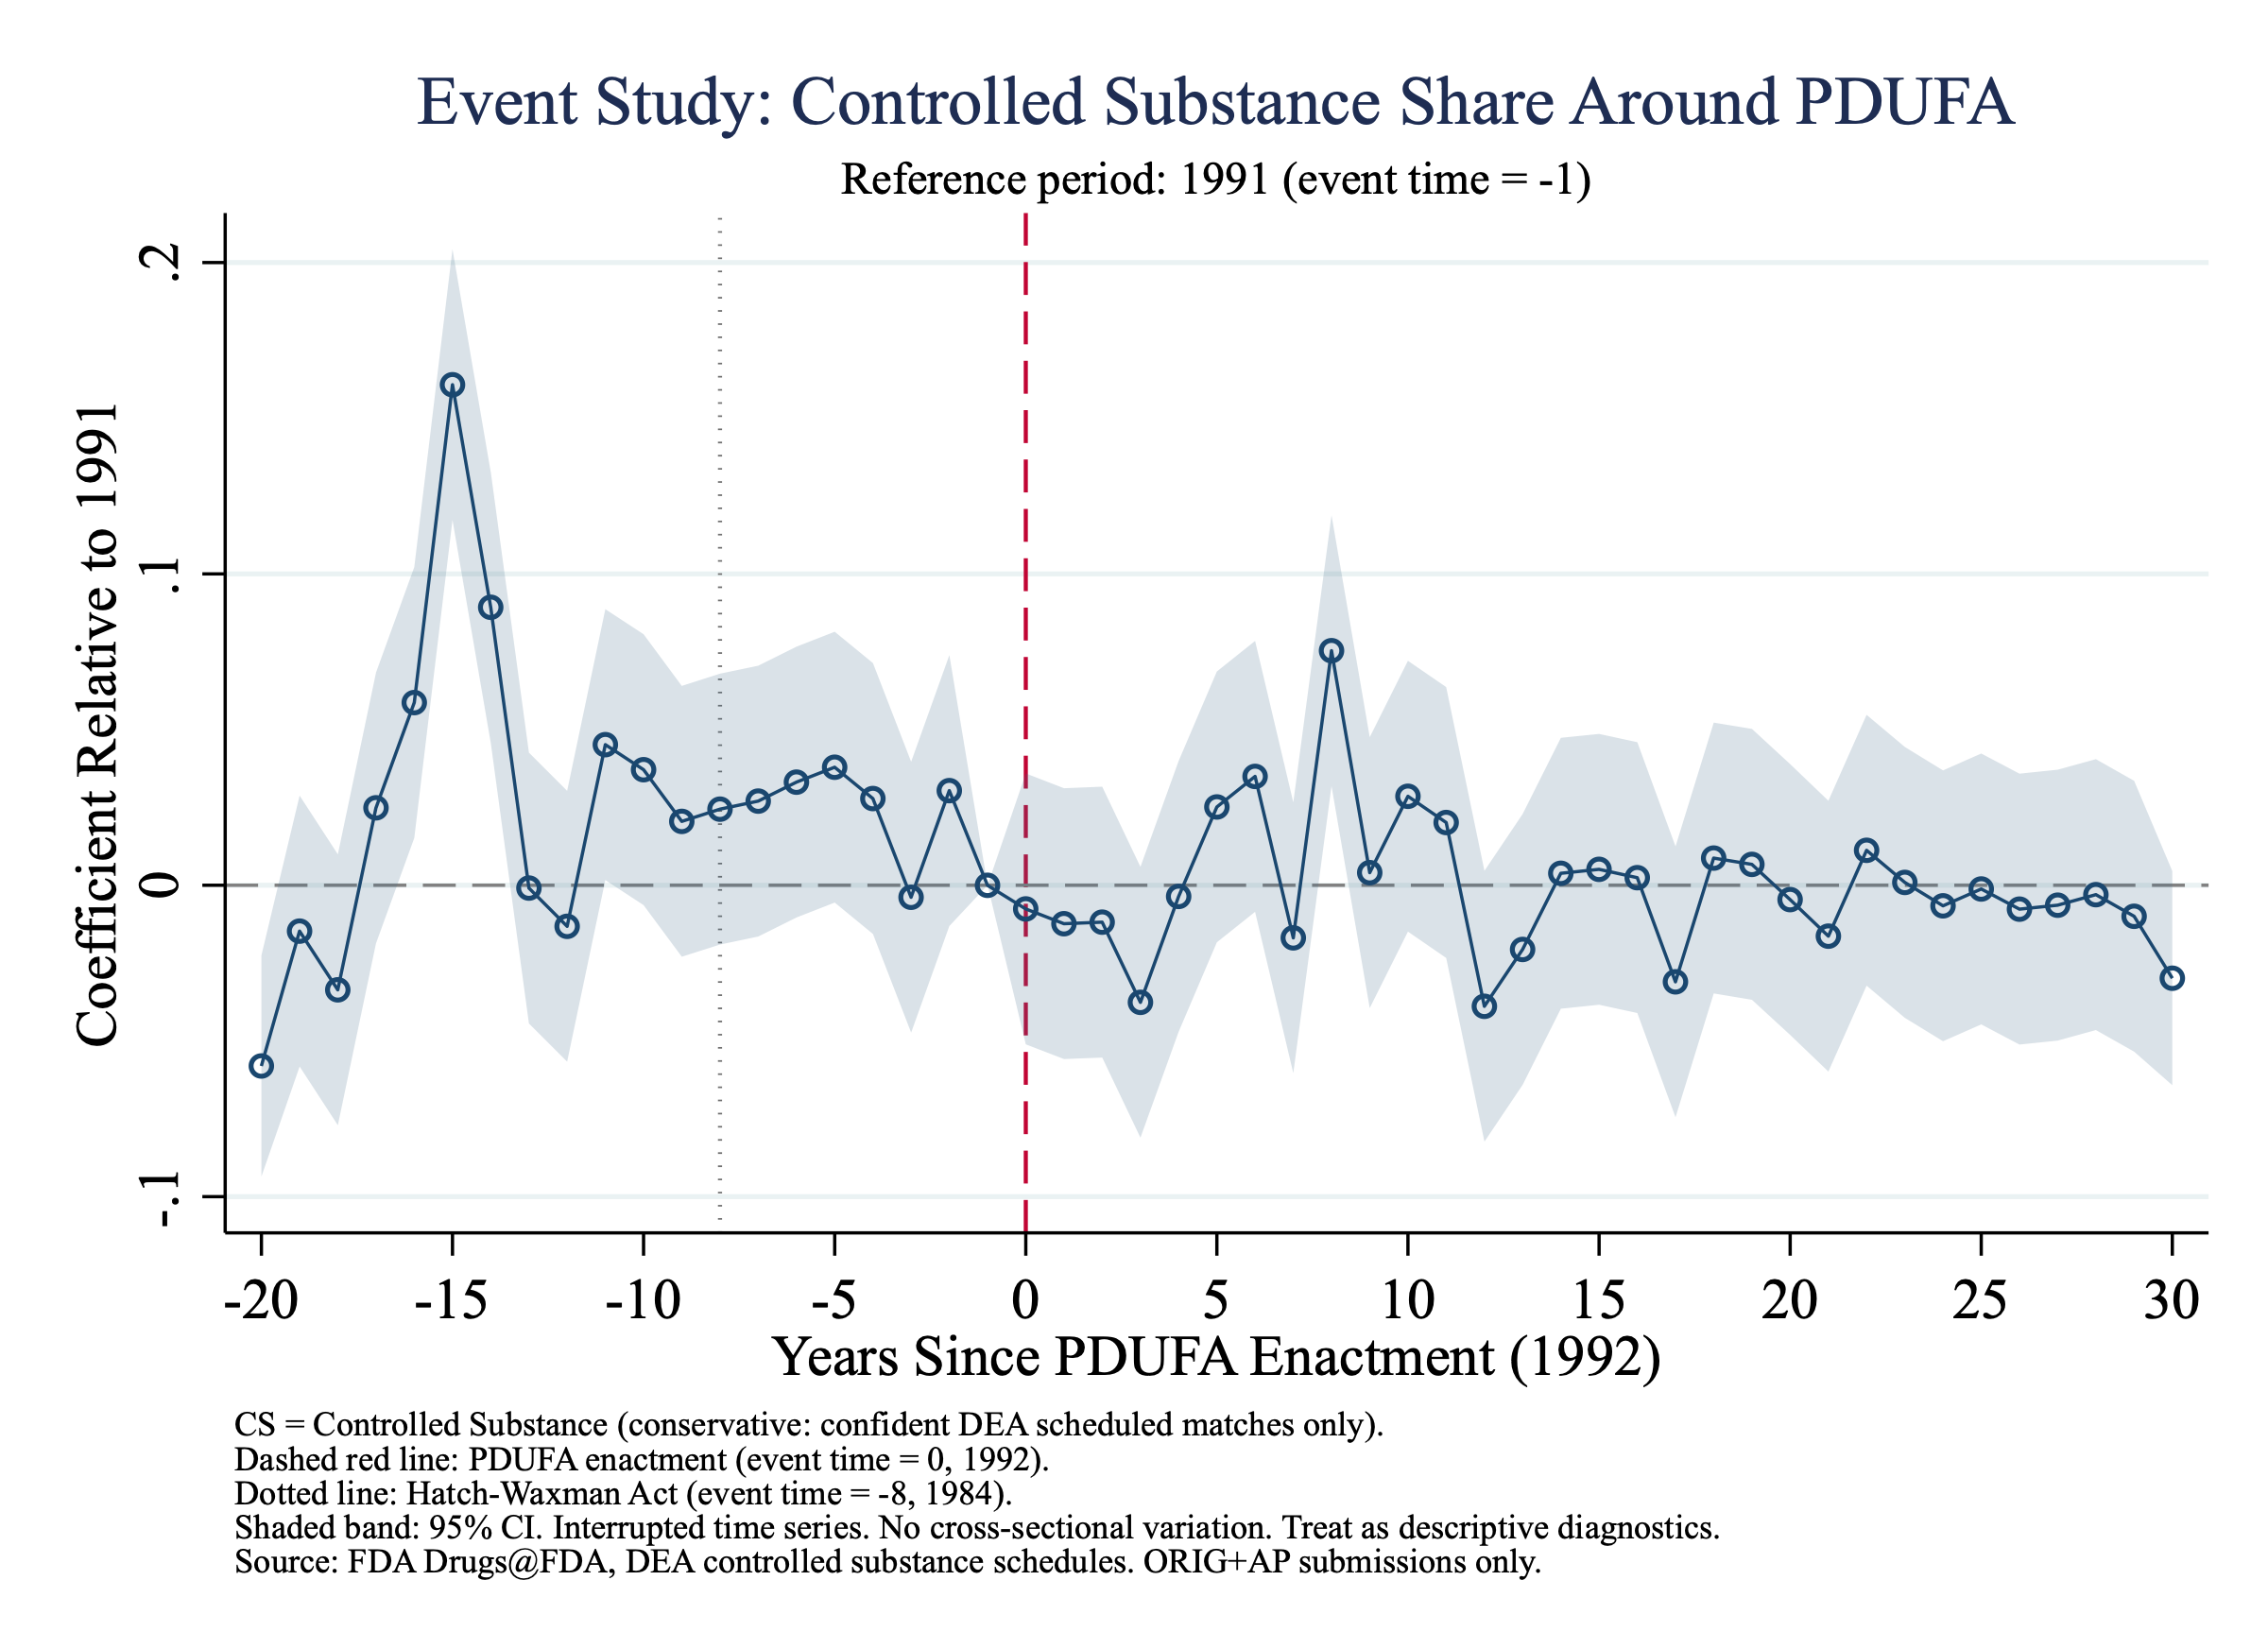
\includegraphics[width=\textwidth]{event_study_cs_share.png}
  \end{center}
  \vfill
  \src{No visible break at event time 0. Pre-event coefficients are not flat
  (spike at $\approx -15$, likely reflecting 1970s scheduling activity).
  Post-event coefficients hover near zero or slightly negative. Wide CIs.}
\end{frame}

\begin{frame}[t]{Event Study --- Log CS Counts}
  \begin{center}
    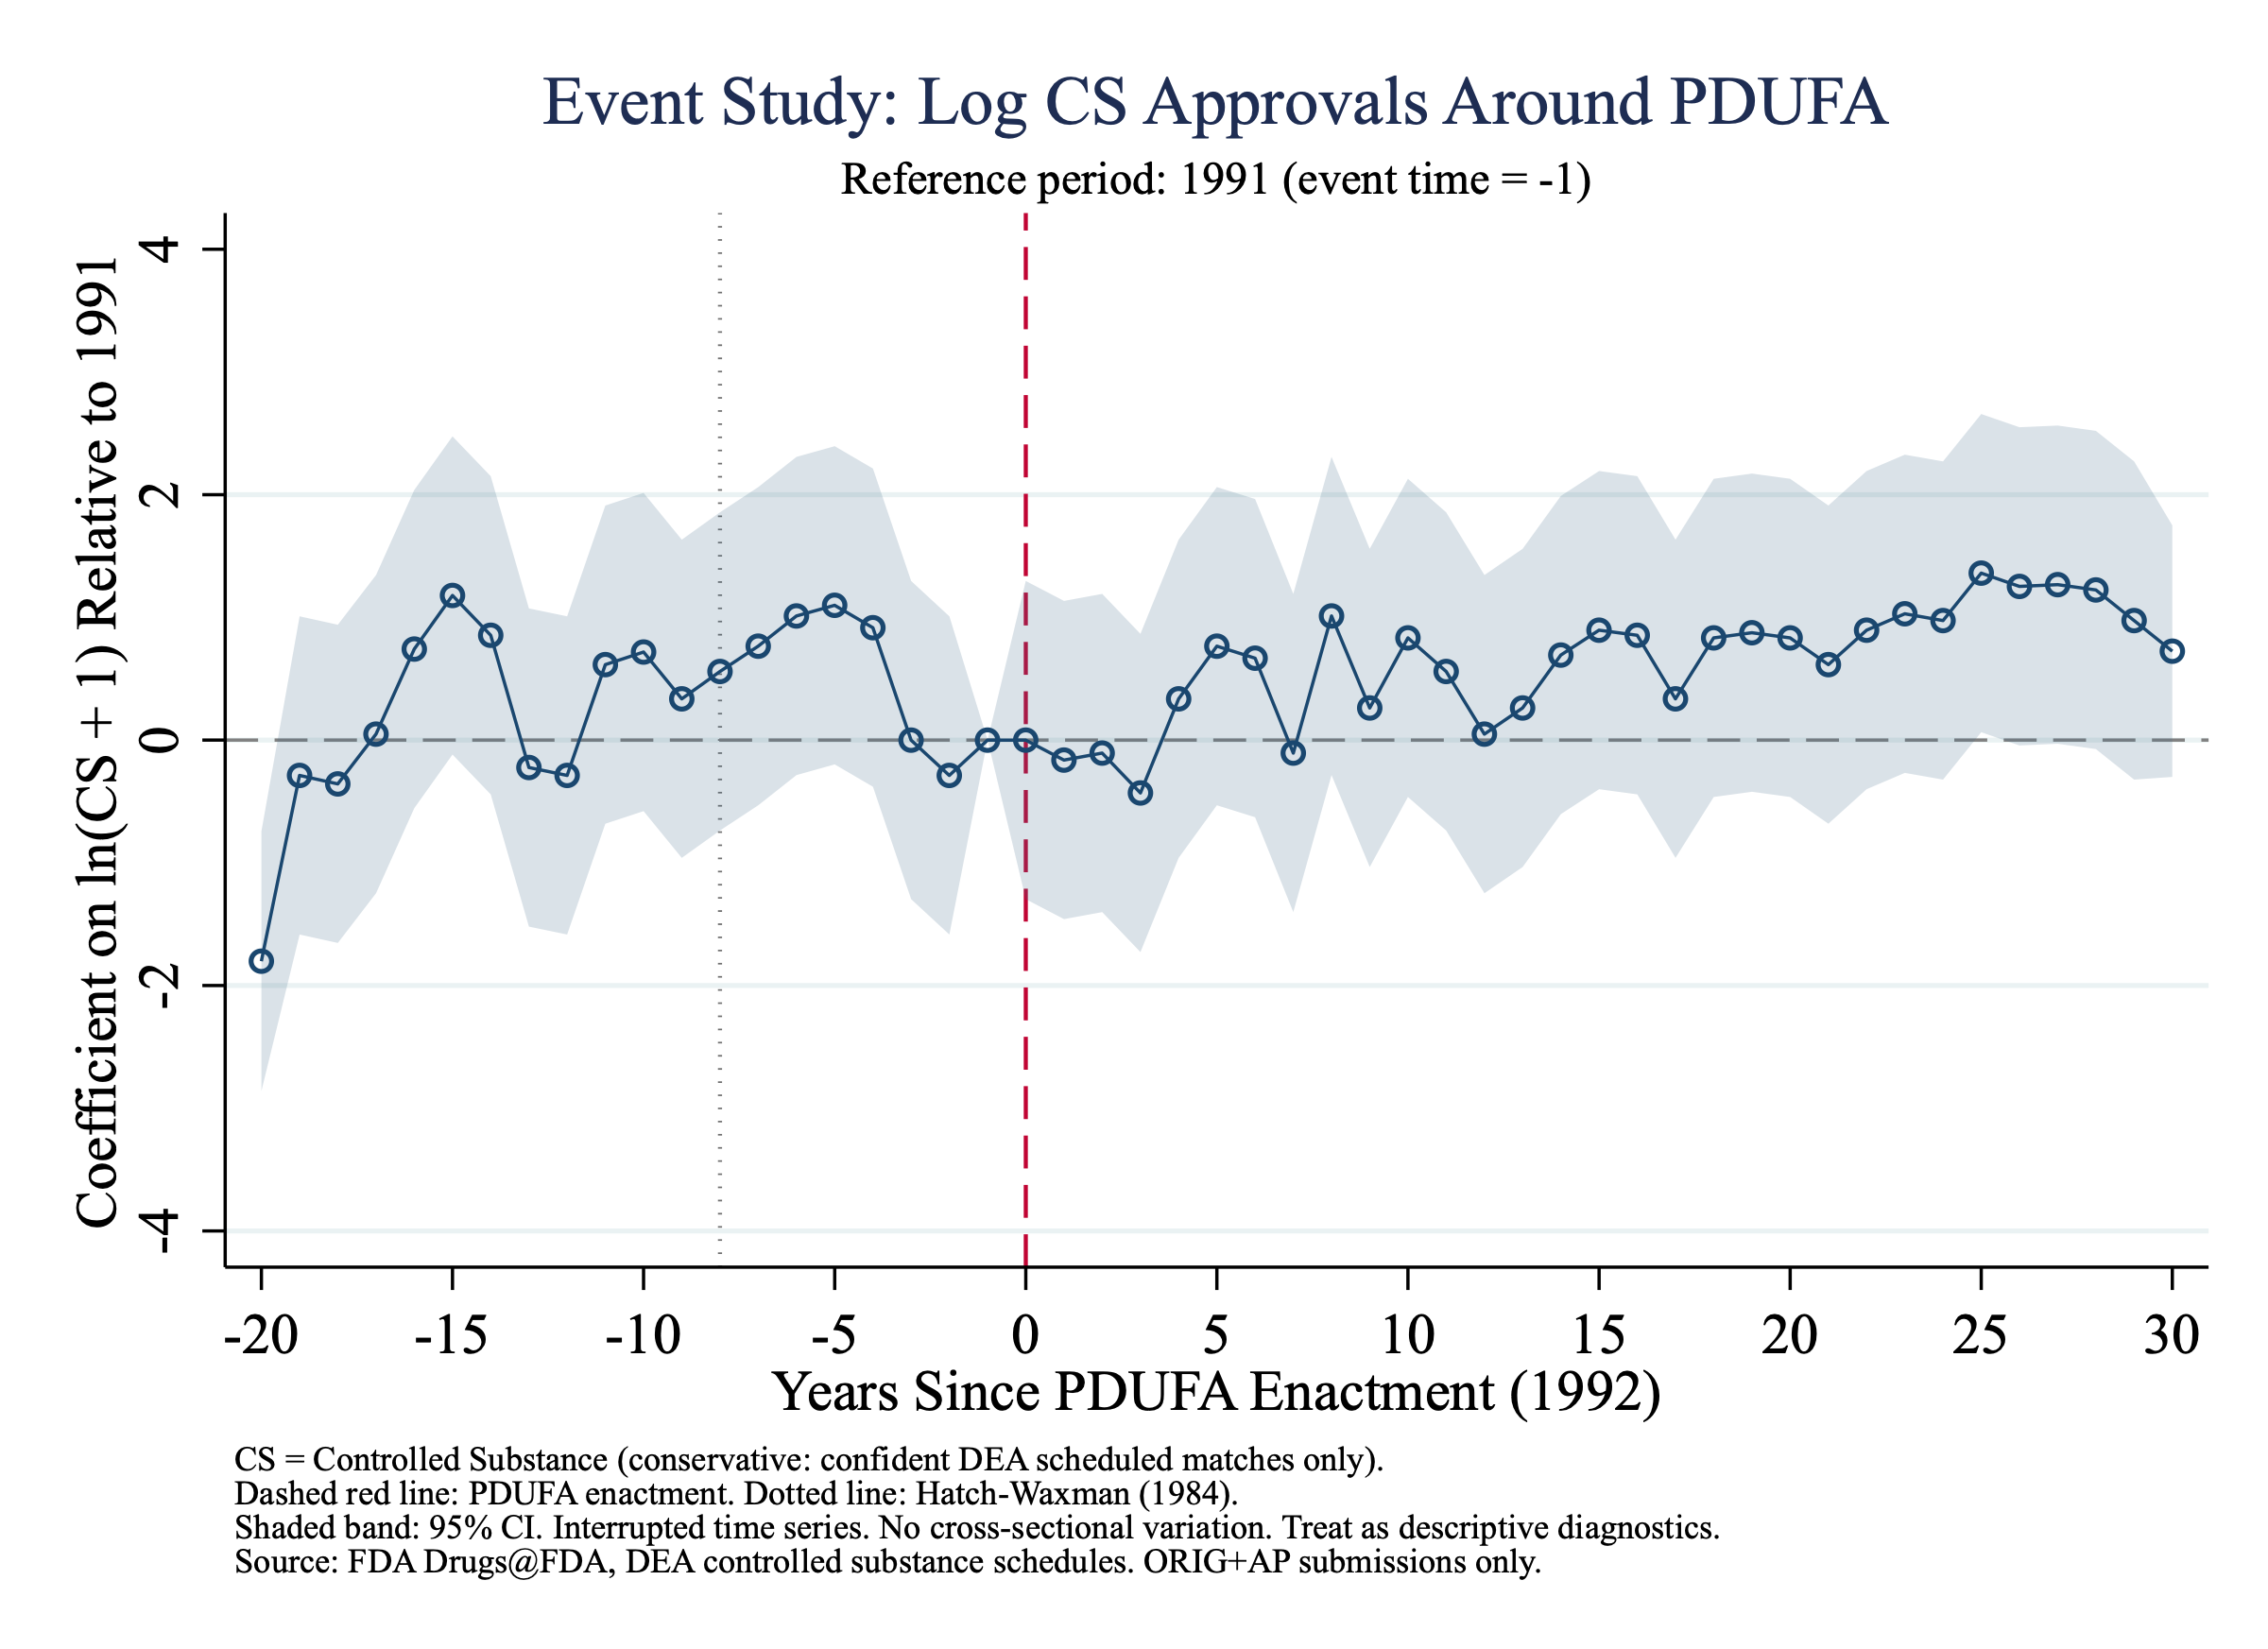
\includegraphics[width=\textwidth]{event_study_ln_cs.png}
  \end{center}
  \vfill
  \src{CS = Controlled Substance. Log CS approvals trend upward over time,
  but growth is gradual with no sharp break at 1992.
  Wide confidence intervals throughout --- only $\approx$55 annual observations.}
\end{frame}

\begin{frame}[t]{Event Study --- CS vs.\ Non-CS Log Counts}
  \begin{center}
    
\includegraphics[width=\textwidth]{event_study_ln_cs_vs_noncs.png}
  \end{center}
  \vfill
  \src{Both CS and non-CS approvals grow after PDUFA and track each other
  through the 1990s--2000s. Non-CS pulls ahead after $\approx$2005,
  driving the declining CS share. The divergence is \textbf{not at 1992}.}
\end{frame}

\begin{frame}[t]{Event Study --- NDA-Only CS Share}
  \begin{center}
    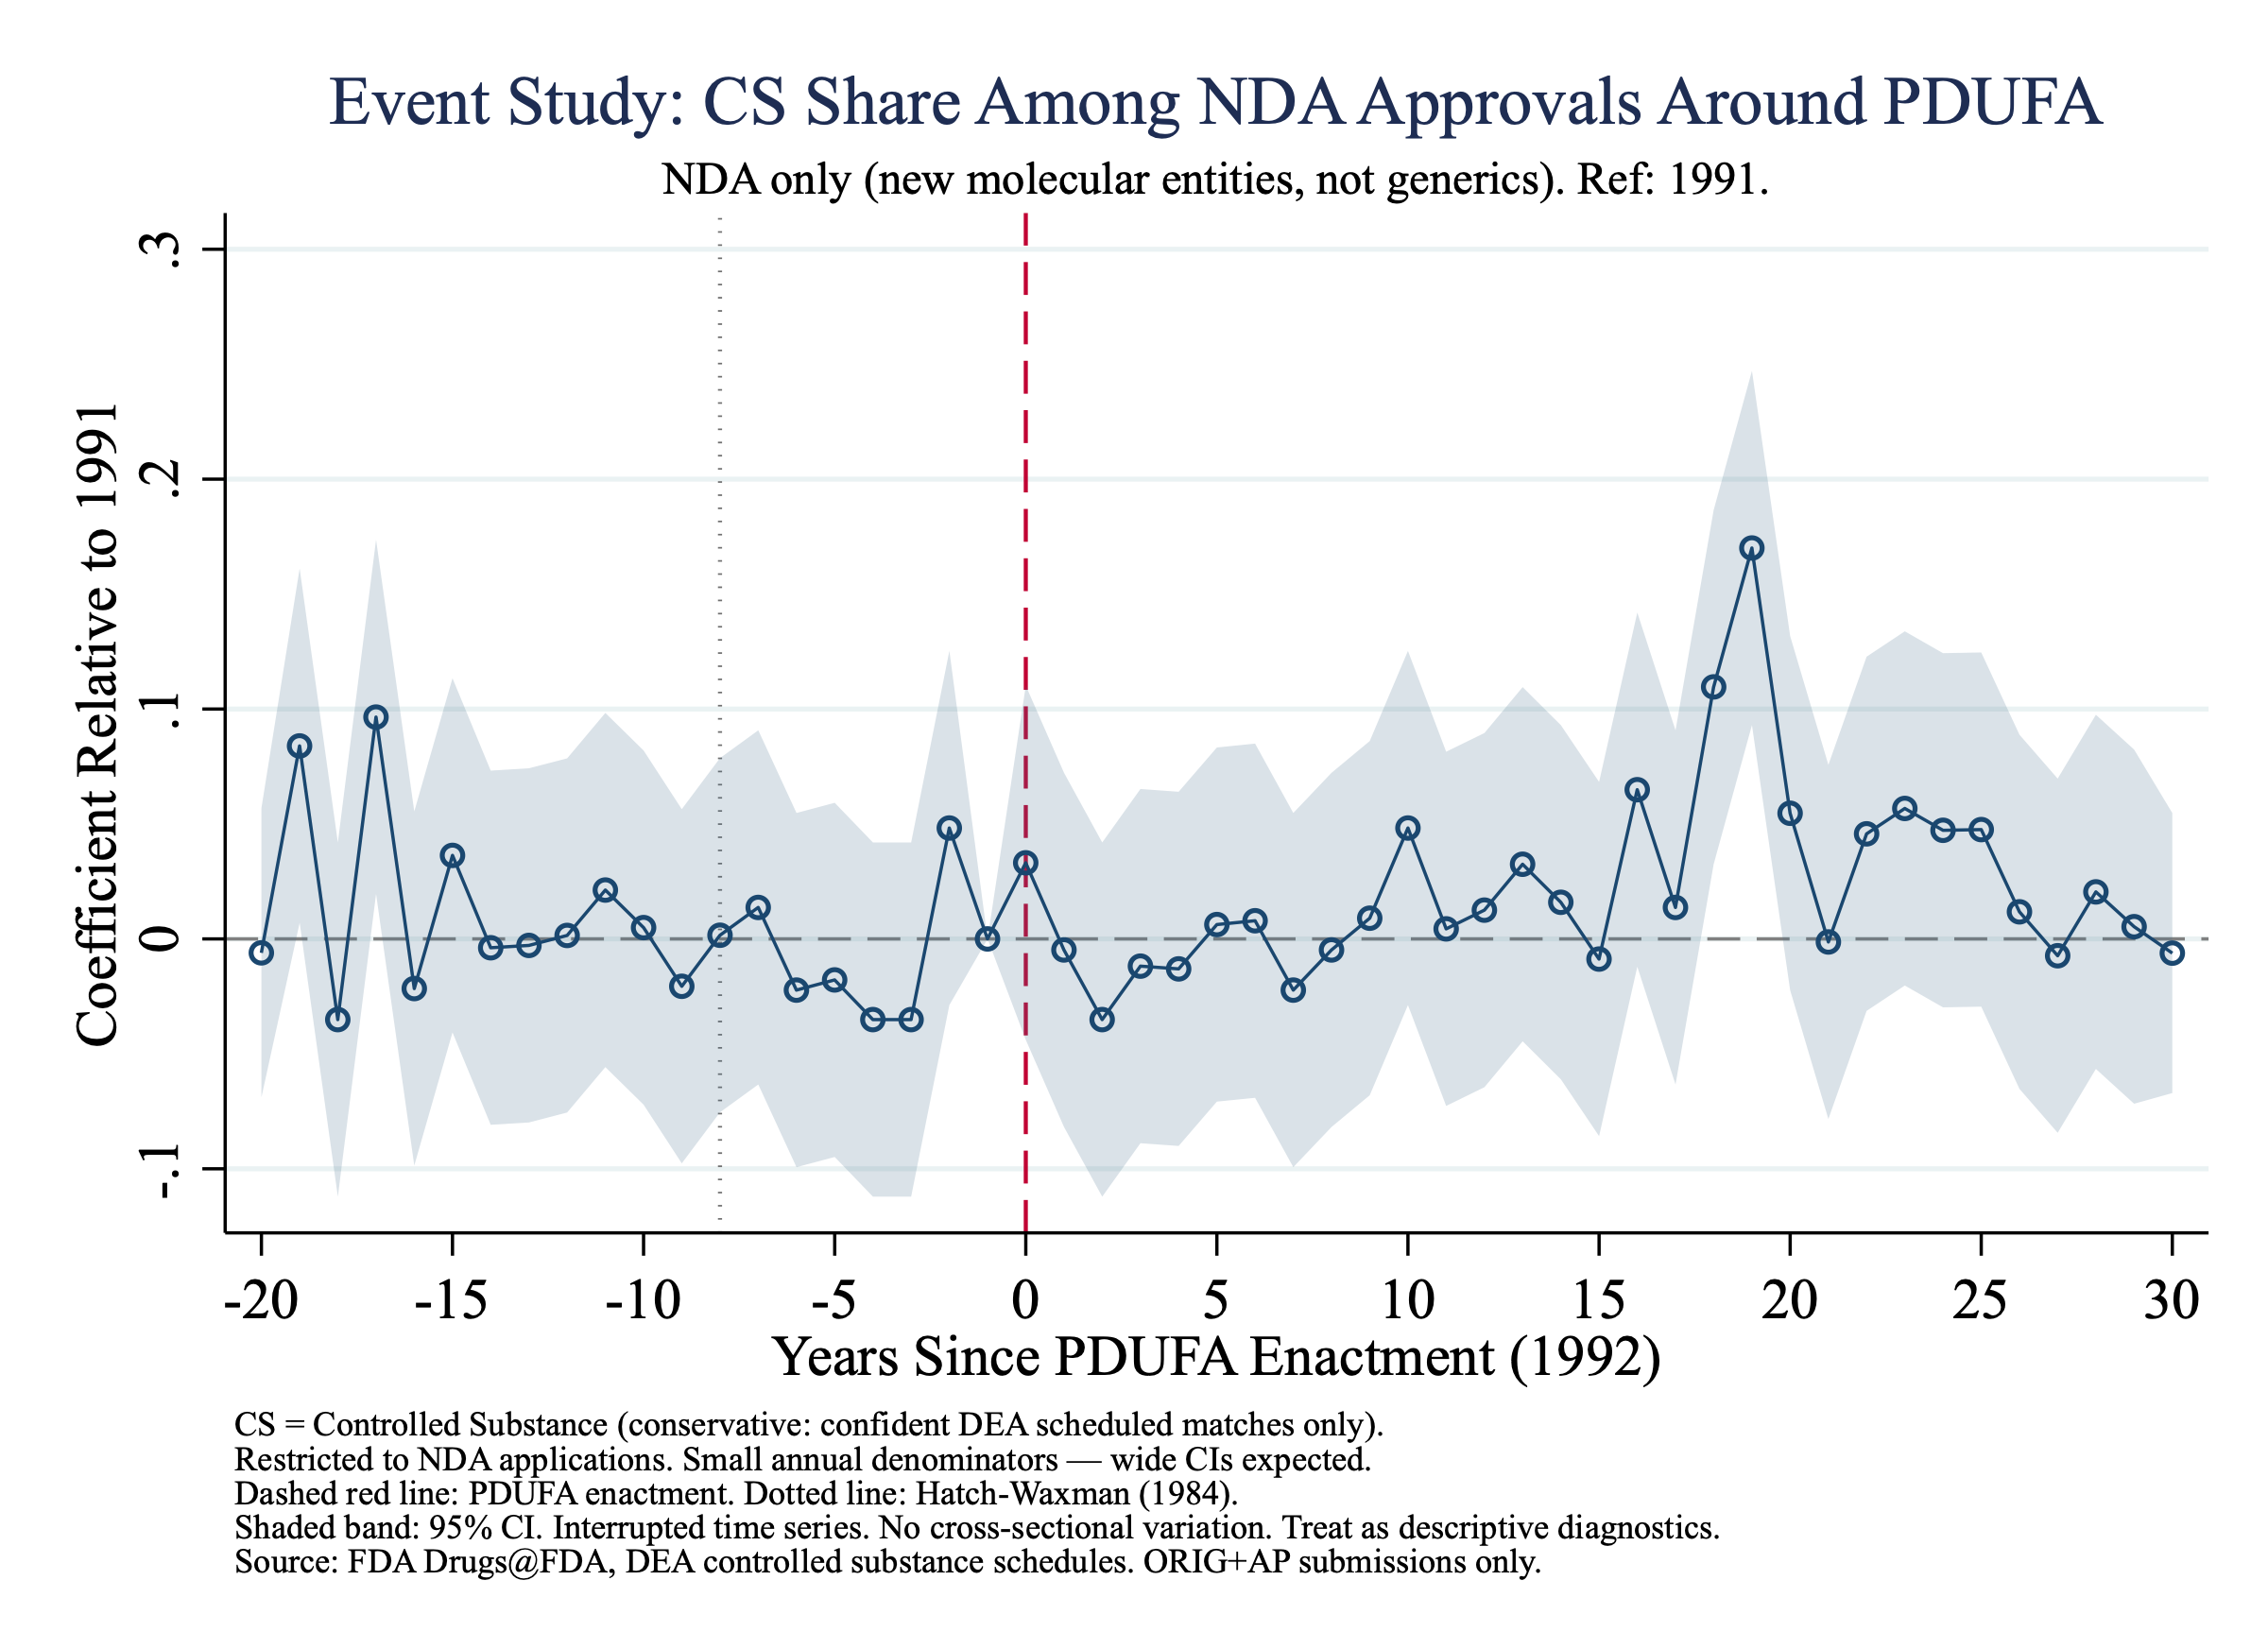
\includegraphics[width=\textwidth]{event_study_cs_share_nda.png}
  \end{center}
  \vfill
  \src{Confidence intervals span 30+ percentage points. Pure noise.
  Sample too small ($\approx$30--50 NDAs/year) to detect anything meaningful.
  Cannot draw conclusions from this specification.}
\end{frame}

\begin{frame}[t]{Summary Figure: Raw Series with Pre/Post Means}
  \begin{center}
    
\includegraphics[width=\textwidth]{event_study_summary.png}
  \end{center}
  \vfill
  \src{CS = Controlled Substance. Raw CS share with pre-PDUFA mean
  ($\approx$9.6\%, 1970--1992) and post-PDUFA mean ($\approx$7.3\%,
  1993--2025). The post-PDUFA average is \textbf{lower}, not higher.}
\end{frame}

\begin{frame}[t]{Parametric Results: Did the CS Share Shift at PDUFA?}
  Annual panel, 56 observations (1970--2025). Outcome: CS share of total approvals.

  \medskip
  \textbf{Model A --- Simple level shift:}
  \[
    \text{CS Share}_t = \beta_0 + \beta_1 \cdot \mathbf{1}[\text{Post-PDUFA}_t] + \varepsilon_t
  \]

  \begin{center}
  \begin{tabular}{lcccc}
    \hline
    & Coef. & Std.\ Err. & $p$-value & $R^2$ \\
    \hline
    Post-PDUFA ($\beta_1$) & $-0.020$ & $0.010$ & $0.052$ & \\
    Constant ($\beta_0$)   & $\phantom{-}0.096$ & $0.008$ & $0.000$ & $0.068$ \\
    \hline
  \end{tabular}
  \end{center}

  \medskip
  \textit{The average CS share was 9.6\% before PDUFA and about 2 pp lower
  after. Marginally significant ($p = 0.052$).
  The CS share \textit{fell} --- it did not rise.}
\end{frame}

\begin{frame}[t]{Parametric Results: Controlling for Trend and Slope Change}
  \textbf{Model B --- Level shift + linear time trend:}
  \[
    \text{CS Share}_t = \beta_0 + \beta_1 \cdot \mathbf{1}[\text{Post}_t]
                        + \beta_2 \cdot \text{Year}_t + \varepsilon_t
  \]
  \begin{center}
  \begin{tabular}{lccc}
    \hline
    & Coef. & Std.\ Err. & $p$-value \\
    \hline
    Post-PDUFA ($\beta_1$) & $-0.015$ & $0.019$ & $0.446$ \\
    Year ($\beta_2$)       & $-0.0002$ & $0.0006$ & $0.759$ \\
    \hline
    \multicolumn{4}{l}{$R^2 = 0.070$. $N = 56$.} \\
  \end{tabular}
  \end{center}

  \smallskip
  \textbf{Model C --- Level shift + trend + slope change:}
  \[
    \text{CS Share}_t = \beta_0 + \beta_1 \cdot \mathbf{1}[\text{Post}_t]
                        + \beta_2 \cdot \text{Year}_t
                        + \beta_3 \cdot (t - 1992) \times \mathbf{1}[\text{Post}_t]
                        + \varepsilon_t
  \]
  \begin{center}
  \begin{tabular}{lccc}
    \hline
    & Coef. & Std.\ Err. & $p$-value \\
    \hline
    Post-PDUFA ($\beta_1$)  & $-0.025$ & $0.019$ & $0.205$ \\
    Year ($\beta_2$)         & $\phantom{-}0.002$ & $0.001$ & $0.128$ \\
    Slope change ($\beta_3$) & $-0.003$ & $0.001$ & $0.054$ \\
    \hline
    \multicolumn{4}{l}{$R^2 = 0.135$. $N = 56$.} \\
  \end{tabular}
  \end{center}

  \smallskip
  \textit{Once we control for trend, the PDUFA shift is statistically zero.
  The slope change ($\beta_3 = -0.003$, $p = 0.054$) suggests a marginally
  significant \textit{downward} acceleration --- the \textbf{opposite} direction
  of the hypothesis.}
\end{frame}

\begin{frame}[t]{Parametric Results: Log Counts}
  \textbf{Model D --- Log CS approvals, trend + slope change:}
  \[
    \ln(\text{CS}_t + 1) = \beta_0 + \beta_1 \cdot \mathbf{1}[\text{Post}_t]
                           + \beta_2 \cdot \text{Year}_t
                           + \beta_3 \cdot (t - 1992) \times \mathbf{1}[\text{Post}_t]
                           + \varepsilon_t
  \]
  \begin{center}
  \begin{tabular}{lccc}
    \hline
    & Coef. & Std.\ Err. & $p$-value \\
    \hline
    Post-PDUFA ($\beta_1$)  & $-0.704$ & $0.311$ & $0.028$ \\
    Year ($\beta_2$)         & $\phantom{-}0.070$ & $0.018$ & $0.000$ \\
    Slope change ($\beta_3$) & $-0.040$ & $0.021$ & $0.064$ \\
    \hline
    \multicolumn{4}{l}{$R^2 = 0.409$. $N = 56$.} \\
  \end{tabular}
  \end{center}

  \medskip
  \textit{CS approvals grow over time ($\beta_2 > 0$, $p < 0.001$). But the
  post-PDUFA level shift is \textit{negative} ($\beta_1 = -0.704$, $p = 0.028$)
  --- CS counts were \textit{below} trend right after PDUFA. The slope change
  is also negative: CS approval growth \textit{slowed} after 1992.}

  \medskip
  \begin{block}{Bottom line}
    \textbf{Across all four models: no evidence that PDUFA increased controlled
    substance approvals, whether measured as a share or in log counts.}
  \end{block}
\end{frame}

%% =============================================================================
\section{Problems and Limitations}
%% =============================================================================

\begin{frame}[t]{Problem 1: DEA Linkage Is Retroactive}
  \begin{itemize}
    \item We apply \textbf{current (2026) DEA scheduling} to drugs approved
          decades ago
    \item A drug approved in 1975 may not have been scheduled at approval ---
          or may have had a different schedule
    \item Scheduling status changes: drugs get rescheduled up or down (e.g.,
          hydrocodone combination products moved II $\to$ III $\to$ II)
    \item We have \alert{no historical scheduling data}
    \item \textbf{Consequence:} the level of the CS share in any given year may
          be mismeasured; changes over time may partly reflect DEA
          rescheduling events rather than changes in approval composition
    \item Pre-event spike ($\approx$event time $-15$, i.e.\ $\approx$1977)
          may reflect a historical scheduling wave that is now retroactively
          coded into our sample
  \end{itemize}
\end{frame}

\begin{frame}[t]{Problem 2: The Denominator Problem Is Fundamental}
  \begin{itemize}
    \item Total approvals quadrupled after PDUFA, driven by the ANDA explosion
    \item Even if CS approvals grew, the \textit{share} falls if non-CS
          approvals grow faster
    \item The share-based outcome \textbf{conflates numerator and denominator
          dynamics}
    \item Log counts partially address this, but do not cleanly separate
          ``more CS drugs'' from ``more drugs overall''
    \item The ideal approach: model CS and non-CS entry separately; test for
          \textit{differential} growth rates
    \item This is not merely a scaling issue --- it is a question about what
          the economically meaningful outcome measure is
    \item \alert{Candidate reframing:} study the absolute supply of controlled
          substances (level) rather than their share of approvals
  \end{itemize}
\end{frame}

\begin{frame}[t]{Problem 3: Sample Mixes New Molecular Entities with Generics}
  \begin{itemize}
    \item An ANDA for generic oxycodone $\ne$ an NDA for a novel opioid
    \item The PDUFA-as-incentive hypothesis applies to \textbf{NDAs}
          (new drug development decisions by innovator firms)
    \item But \textbf{86.6\%} of CS approvals are ANDAs --- generic copies
          of existing controlled substances
    \item NDA-only analysis is conceptually cleaner but statistically
          underpowered ($\approx$30--50 NDAs/year; CIs span 30 pp)
    \item \alert{What the data actually describe:} a
          \textbf{generic-drug proliferation story}, not an innovation story
    \item More Schedule II and IV generic copies of existing brand-name
          controlled substances entering the market after Hatch-Waxman
    \item That is a \textbf{Hatch-Waxman story}, not a PDUFA story
  \end{itemize}
\end{frame}

\begin{frame}[t]{Problem 4: Hatch-Waxman (1984) Confounds the Pre-Period}
  \begin{itemize}
    \item Hatch-Waxman created the entire ANDA pathway for generics in 1984
    \item This is arguably the \textbf{larger structural change} in the
          approval landscape --- bigger than PDUFA
    \item The pre-PDUFA period (1970--1992) \textit{includes} this massive
          shock 8 years before our treatment
    \item Pre-event coefficients in the event study are \textbf{not flat} ---
          there is a visible pre-trend that likely reflects Hatch-Waxman
          dynamics
    \item We cannot cleanly separate Hatch-Waxman effects from PDUFA effects
          with this design
    \item \alert{The two policies are bundled in calendar time} and both affect
          the composition of the approval pool
    \item One mitigation: restrict to NDAs only; but then we lose power
  \end{itemize}
\end{frame}

\begin{frame}[t]{Problem 5: No Correction for Serial Correlation}
  \begin{itemize}
    \item Annual CS share is almost certainly \textbf{autocorrelated} --- drug
          approvals have multi-year regulatory lags, and scheduling waves
          affect multiple years at once
    \item OLS standard errors do not account for this; CIs may be too narrow
    \item Newey-West (HAC) standard errors with lag $\approx 3$ would be
          appropriate for a paper-facing version
    \item With only $\approx$55 annual observations, HAC corrections have
          limited small-sample reliability in any case
    \item \textbf{Qualitative conclusion is likely unchanged} (most point
          estimates are small or near zero regardless), but formal inference
          is imprecise
    \item This is noted throughout the do-file but not yet corrected in the
          current output
  \end{itemize}
\end{frame}

\begin{frame}[t]{Problem 6: Single National Time Series $\ne$ Causal Design}
  \begin{itemize}
    \item \textbf{No untreated units.} No cross-sectional variation in
          treatment timing. Cannot construct a counterfactual.
    \item This is an \textbf{interrupted time series} --- the weakest
          quasi-experimental design
    \item Any contemporaneous shock is confounded with PDUFA:
          \begin{itemize}
            \item Changes in DEA scheduling practice in the 1990s
            \item Pharmaceutical R\&D portfolio shifts
            \item Opioid crisis and related regulatory responses
            \item Economic cycles affecting generic entry timing
          \end{itemize}
    \item Miller (2023, JEP): with only treated units and a common event
          date, treatment effect identification requires very strong
          counterfactual assumptions
    \item \alert{Bottom line:} even if we observe a post-1992 change, we
          cannot attribute it to PDUFA with any confidence
  \end{itemize}
\end{frame}

%% =============================================================================
\section{Where This Leaves the Thesis}
%% =============================================================================

\begin{frame}[t]{What We Can Honestly Conclude}
  \begin{itemize}
    \item PDUFA did \textbf{not} increase the \textit{share} of FDA-approved
          drugs that are controlled substances --- the share declined
    \item Raw \textit{counts} of CS approvals tripled (from $\approx$13 to
          $\approx$41/year), but this growth was proportional to or slower
          than overall approval growth
    \item The CS approval increase is concentrated in
          \textbf{Schedule II generics} filed through the ANDA pathway
    \item Top sponsors are all generic manufacturers; no innovator firms in
          the top 20
    \item \alert{No evidence that PDUFA created differential incentives for
          controlled substance development}
    \item The data describe a Hatch-Waxman + generic proliferation story,
          not a PDUFA story
  \end{itemize}
\end{frame}

\begin{frame}[t]{Revised Framing of the Question}
  \begin{block}{Original framing}
    ``Did PDUFA's user fee structure incentivize more controlled substance
    approvals?''
  \end{block}

  \medskip
  \textbf{Problems with this framing:}
  \begin{itemize}
    \item User fees are uniform --- not drug-type-specific
    \item ANDAs (86.6\% of CS approvals) weren't covered by PDUFA until 2012
    \item The composition margin shows no positive shift at 1992
  \end{itemize}

  \medskip
  \begin{block}{Weaker but potentially defensible framing}
    ``Did PDUFA-era regulatory acceleration, by increasing overall FDA
    throughput, lead to greater \textit{absolute supply} of controlled
    substances --- even without changing the composition?''
  \end{block}

  \medskip
  The data suggest even this is better attributed to Hatch-Waxman than PDUFA.
\end{frame}

\begin{frame}[t]{Potential Paths Forward}
  \begin{enumerate}
    \item \textbf{Shift from composition to supply:} 41 CS approvals/year vs.\
          13 may matter for downstream outcomes (diversion, misuse) even if
          the share didn't change
    \item \textbf{Study GDUFA (2012):} a natural experiment specifically
          targeting generic drug user fees --- the pathway that dominates CS
          approvals
    \item \textbf{Fix the DEA linkage:} obtain historical scheduling data
          (DEA Orange Book archives, Federal Register notices)
    \item \textbf{Link to downstream outcomes:} ARCOS (retail distribution),
          CDC WONDER (overdose mortality), NFLIS (drug seizure data)
    \item \textbf{Narrow the question:} focus on Schedule II opioids or
          stimulants specifically, not all CS
    \item \textbf{Intensive margin:} study \textit{review time} for CS vs.\
          non-CS drugs under PDUFA, rather than approval composition
    \item \textbf{Pivot the question entirely} --- discuss
  \end{enumerate}
\end{frame}

\begin{frame}[t]{Open Questions for Discussion}
  \begin{enumerate}
    \item Is the \textbf{null result on composition} itself a
          publishable/interesting finding? (``PDUFA didn't change CS share
          because the mechanism doesn't apply to generics'')
    \item Should the thesis pivot to studying \textbf{absolute supply growth}
          rather than composition?
    \item Is \textbf{GDUFA (2012)} a more tractable policy shock? What
          identification challenges does it bring?
    \item What downstream data would make the ``supply $\to$ misuse''
          connection credible? Is ARCOS accessible?
    \item Is there a better identification strategy that could address the
          Hatch-Waxman confound?
    \item Should the thesis \textbf{pivot the question entirely}? If so,
          toward what? Opioid prescribing? Generic entry timing? Something
          else entirely?
  \end{enumerate}
\end{frame}

%% =============================================================================
\section{Conclusion}
%% =============================================================================

\begin{frame}[t]{Thank You}
  \begin{center}
    \Large Thank you \\[1em]
    \normalsize Questions and feedback welcome
  \end{center}

  \bigskip
  \begin{block}{Summary}
    \begin{itemize}
      \item Data built, DEA linkage built, descriptive results complete
      \item First-pass event study complete
      \item Core hypothesis (PDUFA $\to$ more CS approvals as share) not
            supported by the data
      \item The CS story is a generics/Hatch-Waxman story, not a PDUFA story
      \item Many open questions --- feedback on paths forward most useful
    \end{itemize}
  \end{block}

  \bigskip
  \src{All code, data, and figures available in the thesis repository at
  \texttt{/Users/alexdelatorre/Desktop/econ580-thesis}.}
\end{frame}

\end{document}
